\documentclass{template/openetcs_article}
\usepackage[utf8x]{inputenc}
\usepackage{color}
\usepackage{lipsum,url}
\graphicspath{{./template/}{.}{./images/}}
\begin{document}
\frontmatter
\project{openETCS}

%Please do not change anything above this line
%============================
% The document metadata is defined below

%assign a report number here
\reportnum{OETCS/WP7/D01}

%define your workpackage here
\wp{Work-Package 3a: ``Toolchain''}

%set a title here
\title{openETCS Toolchain WP Description of Work}

%set a subtitle here
%\subtitle{Revision}

%set the date of the report here
\date{October 2012\\Revised October 2012}
\date{\today}

%define a list of authors and their affiliation here

\author{Michael Jastram}

\affiliation{WP7 Leader}

\author{Marielle Petit-Doche (interim)}

\affiliation{WP7.1 Task Leader (Primary Tool Chain Analyses and Recommendations)}
  
\author{Marielle Petit-Doche}

\affiliation{WP7.2 Task Leader (Secondary Tools Analyses and Recommendations)}
  
\author{Jan Peleska}

\affiliation{WP7.3 Task Leader (Define and Develop Tool Chain)}

\author{Jonas Helming}

\affiliation{WP7.4 Task Leader (Develop Open Source Ecosystem)}

\author{WP7 participants}

\affiliation{OpenETCS}
    
% define the coverart
\coverart[width=350pt]{chart}

%define the type of report
\reporttype{Description of work}


\begin{abstract}
%define an abstract here
This document contains the description of work planned for WP7.  This revision is necessary, as the workpackage from original ITEA proposal was split.  This document will be the foundation for a revision of the ITEA proposal.

The revised DoW consists of four chapters for the four Tasks of WP7.

\end{abstract}

%=============================
%Do not change the next three lines
\maketitle
\tableofcontents
%\listoffiguresandtables
\newpage
%=============================

% The actual document starts below this line
%=============================


%Start here





% Makes Marginpars easier to read
\setlength{\marginparwidth}{1in}
\let\oldmarginpar\marginpar
\renewcommand\marginpar[1]{\-\oldmarginpar[\raggedleft\scriptsize #1]%
{\raggedright\scriptsize #1}}

\newcommand{\oldtext}[1]{{Old: \scriptsize #1}}

\newenvironment{inoutput}
{\vspace{2mm}
\noindent
\begin{tabular}{|r|p{.68\linewidth}|l|}
\hline}
{
\hline
\end{tabular}}

\section*{Introduction}

This Work Package will provide the tool chain, based on formal methods, that is necessary to
design, develop, verify and validate the ETCS system. This tool chain will encompass all description levels of the system design from holistic viewpoint to code generation. Specific attention shall be paid to the semantics and the traceability of each part of the chain. The formal specification will be used further for verification and code generation.  Other uses of the formal specification are conceivable.

The tool chain must at least support the following tasks:

\begin{enumerate}
\item Support the writing of the formal ETCS system
  description, which may include a wide range of artefacts, from requirements to actual code (and everything in-between).  To achieve this, it will include elements like means of description (e.g. modelling languages), graphical or textual editors, version management, etc.

\item Support code generation.

\item Support actions like execution, debugging and simulation of some or all elements of the system description.

\item Support the generation of elements that are needed for testing, like test cases, test data, test oracle, test procedure execution, etc.

\item Support the verification and validation of the various artefacts, including the formal ETCS specification against the textual ETCS specification.

% (mj) I took this out, as 50128 is mentioned at the end of this section.
% \item Comply with the EN 50128 requirements to tools.

\item Support tracing of artefacts across all tools and build steps, as needed.

\item Analysis of the system description, like transitions and cooperations between models.
% Several models could be successively performed from system to software level, and at the software level, at least two models could be necessary one for functional specification and one of design.

\item Integrate the tools as needed to support the users as efficient as possible.
 
\end{enumerate}

The tool chain definition will benefit from other R\&D projects and off-the-shelves tools. The semantics of the modelling languages shall be carefully studied.

The first goal of this WP is to identify sets of consistent languages and tools enabling the design of the system.  This will be done in close collaboration with WP2.

In order to be able to progress without depending too much on WP2 requirements and other deliverables, the subtasks shall make use of prototyping in order to gain knowledge regarding the possible modelling languages and tool platforms.  

Compliance with CENELEC standards EN 50126, EN 50128 and EN 50129 could have a
significant impact in terms of workload. Moreover it should be included at the
beginning of the tools development in the Development Plan or in a Safety or
Quality Plan in close collaboration with WP4.

%=======================================================================
\section{Primary Tool Chain Analyses and
           Recommendations}
\label{sec:core_tool}
%=======================================================================

The first task is the primary tool chain analyses and recommendations. It
is concerned with the languages themselves, the tools for authoring, as well as the methods used for formalising the requirements and specifications.

The primary tools will be complemented by secondary tools, as outlined in Section~\ref{sec:supporting_tools}.
Specific attention shall be paid to the semantics and the traceability of each part of the chain.

%This tool chain will encompass all description levels of the system design from holistic viewpoint to code generation.  This task is composed of the following activities:


%\begin{quotation}
%\marginpar{(mj) That's a good idea that supports Stan's idea of using prototypes.}
%(jonasHelming) For both, 1.1 as well as 1.2 it would be helpful to have a reference set of ERTMS requirements from WP2. This should be small sub-set of the specification, but be somehow representative. Using this sub-set would ake it much easier to compare different languages and tools. It can be used as a test set. I think this might be even more useful then detailed requirements for the toolchain, as we have quite some compentence on that in WP7 I think. Of course we will work on the requirements from WP2, but to get startedt with a comparison of existing tools, I think a test set might be the most required piece. Any opinions on that? 
%\end{quotation}

\begin{figure}[!ht]
	\begin{center}
	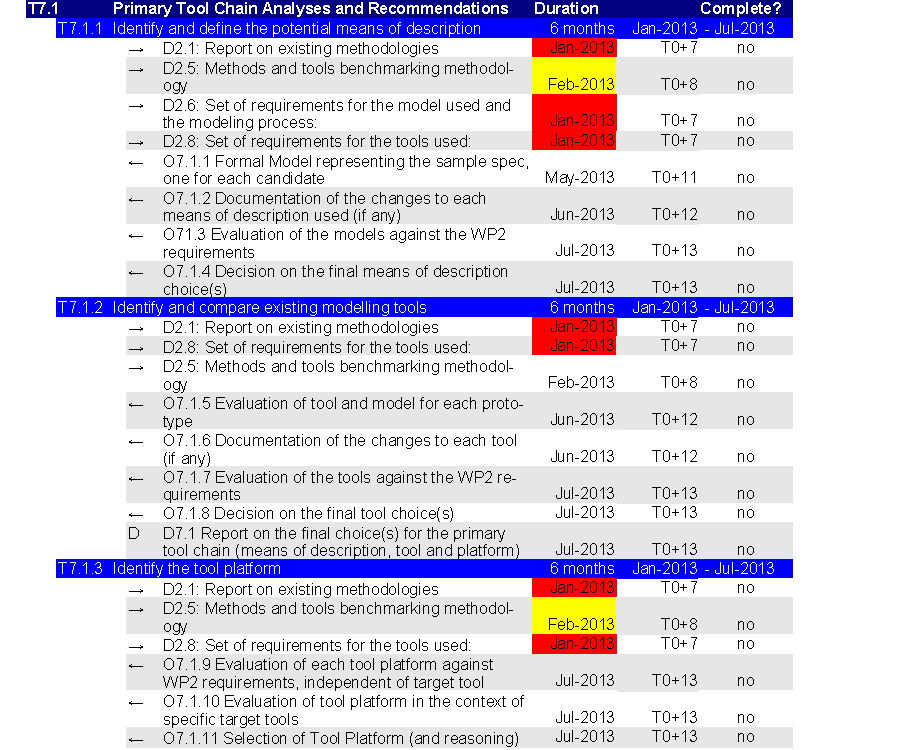
\includegraphics[width=\textwidth,page=1]{project_plan/WP7_Project_Management.pdf}
	\caption{Inputs, Outputs and deliverables for WP7.1}
	\label{fig:wrspm}
	\end{center}
\end{figure}

%-----------------------------------------------------------------------
\subsection{Identify and define the potential means of description}
\label{sec:language}
%-----------------------------------------------------------------------

The goal of this task is to identify the modelling languages that
could fit the requirements associated to the specific needs of ETCS
design and railway norms. Those needs will be defined by tasks of WP2 
(in particular D2.3.1 - Set of requirements on modeling and 
D2.2.1 - Process definition). 
Depending on recommendations of WP2, several languages may
be necessary to handle the different levels of abstraction of the
whole design process.  For each candidate, a small subset of the ERTMS
specification will be modelled. The languages may have to be adapted
in the process. The identification and definition will distinguish
between wide-spectrum modelling languages suitable for a wide variety
of modelling domains such as UML, SysML, B, and domain-specific
languages (DSL) designed and optimised for application in a specific
application domain only.  For wide-spectrum languages their
metamodels\footnote{Recall that metamodels specify the syntax and
  static semantics of a modelling formalism.} will be analysed with
respect to their expressive power and resulting adequateness for
designing ERTMS models.  For DSL candidates the associated
meta-metamodels\footnote{Recall that the meta-metamodel specifies the
  capabilities to define language elements and their static semantics
  in a DSL.}  will be analysed with respect to their capabilities to
support language extensions that may become necessary for novel
releases of the ERTMS specification in the future.  Since no
language is universal (i.e. able to address all aspects of
design needs) the proposed approach is likely to involve several
modelling languages supporting different viewpoints and working at
different levels of abstractions. With this kind of approach, we will
need to check the compatibility of the semantics of the modelling
languages that address overlapping viewpoints. There are two problems
here. First, when dealing with an heterogeneous specification, we need
a common semantical basis to check the compatibility of the
models. More pragmatically, when we deal with two models (expressed in
different languages) that describe the same part of the system, we
need to show that they are consistent with each other. Candidate
languages will be subsequently evaluated against the requirements from
WP2.  If a suitable language is identified, but no partner steps up to
model the prototype, it will not be considered.

%Given that different levels of abstraction have to be addressed in the
%design phase, several languages may be necessary to handle all design
%phases. Here, the semantics of the languages is the key point; it
%shall be accurately adapted to the level of description required in
%each phase of the design.

%\begin{inoutput}
%Input: & WP2: List of suitable languages (based on State of the Art Analysis) & Nov-12 \\
%Input: & WP2: Small subset of ERTMS requirements that is representative & Nov-12 \\
%Input: & Those WP2 Requirements that are sufficient to evaluate a target language & Jan-13 \\
%\hline
%Output: & Formal Model representing the sample spec, one for each candidate & Mar-13 \\
%Output: & Documentation of the changes to each language used (if any) & Mar-13 \\
%Output: & Evaluation of the models against the WP2 requirements & Apr-13 \\
%Output: & Decision on the final language choice(s) & May-13 \\
%\hline
%Deliverable: & Report on the candidate languages 
%(sample model, evaluation against requirements and evolution needed) & Apr-13 \\
%Deliverable: & Report on the final language choice(s) & May-13 \\
%\end{inoutput}

%-----------------------------------------------------------------------
\subsection{Identify and compare existing modelling tools}
\label{sec:tool}
%-----------------------------------------------------------------------

Corresponding to Section~\ref{sec:language}, the objective of this
subtask is the identification of the primary modelling tools 
(analysis and other secondary tools will be the subject of 
Section~\ref{sec:supporting_tools}), 
based on the
analysis from WP2, by using it for the prototyping described in
Section~\ref{sec:language}. 

The experience with the tools will be recorded, and the tools will be
evaluated against the requirements from WP2. In particular, the compliance of
the candidate tools with respect to EN50128 constraints will be investigated.

%\begin{inoutput}
%Input: & WP2: List of suitable tools (based on State of the Art Analysis) & Nov-12 \\
%Input: & Those WP2 Requirements that are sufficient to evaluate the tool & Jan-13 \\
%\hline
%Output: & Experience report for each candidate tool & Apr-13 \\
%Output: & Documentation of the changes to each tool (if any) & Apr-13 \\
%Output: & Evaluation of the tools against the WP2 requirements & May-13 \\
%Output: & Decision on the final tool choice(s) & Jun-13 \\
%\hline
%Deliverable: & Report on the candidate tools 
% (evaluation against requirements and evolution needed) & May-13 \\
%Deliverable: & Report on the final tool choice(s) & Jun-13 \\
%\end{inoutput}



%-----------------------------------------------------------------------
\subsection{Identify the tool platform}
\label{sec:tool_platform}
%-----------------------------------------------------------------------

There is a distinction between tools (Section~\ref{sec:tool}) and tool
platform: The tools are the core that processes the languages, and
typically also have an editor. The tool platform is language
independent, but provides mechanisms to integrate various tools. For
example, Eclipse is a tool platform. The Java Development Tools (JDT)
are an extension to Eclipse that allows working with the Java
programming language.

As the toolchain will consist of many tools that must work together
seamlessly, it should be analysed independently from the tools. A tool
will typically suggest a certain tool platform. The aim of this task
is the identification of a tool platform for each candidate tool from
Section~\ref{sec:tool}. In particular, the platform should provide an
suitable to interface (e.g.~XML or JSON definition) to facilitate data
exchanges between the various tools of the toolchain.

Several levels of interoperability can be supported by the
toolchain. For instance, in Eclipse, the most basic level
provides support for plugins (OSGi); that is the ability to have
several tools inside a common platform. In the project, we will also
need support for interoperability at the data level, which can be
found in the Eclipse world with the Modeling Framework; that is the
ability to have tools that converse/interact using a standardized
(low-level) syntax. Finally, we could also require interoperability at
a ``semantical'' level---for example with support for linking objects
in different modeling languages---or ask for more basic services, such
as serialization and versioning. We believe that, for the project, we
at least need interoperability at the data level. Please note that this 
example is indicative and does not represent a technology decision.

As with modelling tools, tool platforms will be evaluated against WP2 
requirements, including in particular compliance against EN50128 constraints.

%\begin{inoutput}
%Input: & List of target platforms, based on the tools being evaluated (\ref{sec:tool}) & Nov-12 \\
%& Those WP2 Requirements that are sufficient to evaluate a target language & Dec-12 \\
%\hline
%Output: & Evaluation of each tool platform against WP2 requirements, independent of target tool & Mar-13 \\
%Output: & Evaluation of tool platform in the context of specific target tools & Apr-13 \\
%Output: & Selection of Tool Platform (and reasoning) & May-13 \\
%\hline
%Deliverable: & Report on candidate tool platform 
%(evaluation against requirements and target tool) & Apr-13 \\
%Deliverable: & Report on Tool Platform Selection & May-13 \\
%\end{inoutput}

%=======================================================================
\section{Secondary Tools Analyses and Recommendations}
\label{sec:supporting_tools}
%=======================================================================

The languages and tools  of the primary chain have to be complemented to support a number of activities that are crucial for the project. The purpose of this task is to compose a list of tools which may be
used in performing or supporting  activities, analyse their
suitability and propose a selection for inclusion in the openETCS tool
basis. This has to be coordinated with 

\begin{itemize}
\item the primary tool chain selection (suitable  tools should be
  available), 
\item the definition of the overall development process, as that defines the steps to be performed and 
\item the safety analyses to  conclude if the proposed tools are suitable to fulfil standard criteria for a certifiable tool chain.
\end{itemize}

The flow of information in the coordination is bidirectional, e.g. the process
steps should ideally be tailored towards realizability with good
support by available tools. Techniques complementing the
tool-supported steps must be included in the process description. 
  
\begin{figure}[!ht]
	\begin{center}
	\includegraphics[width=\textwidth,page=2]{project_plan/WP7_Project_Management.pdf}
	\caption{Inputs, Outputs and deliverables for WP7.2}
	\label{fig:wrspm}
	\end{center}
\end{figure}



%-----------------------------------------------------------------------
\subsection{Identify and define the secondary tools and methods}
%-----------------------------------------------------------------------


The goal of this subtask  is to identify  the secondary methods and tools that could complete the primary tool chain to  achieve the WP2 requirements.

The following activities  have already be identified and detailed in the following sections :

\begin{itemize}
\item Model Transformation, code generation,
\item Requirement traceability
\item Validation and verification
\item Safety analyses Tools
\end{itemize}

%\begin{inoutput}
%Input: & WP2: List of suitable languages (based on State of the Art Analysis) & Nov-12 \\
%Input: & WP2: Small subset of ERTMS requirements that is representative & Nov-12 \\
%Input: & Those WP2 Requirements that are sufficient to evaluate a target language & Jan-13 \\
%Input: & WP2: Definition of the process & Jan-13 \\
%Input: & WP7: Decision of the final choice for the core language & May-13 \\
%\hline
%Output: & Evaluation of secondary tools and methods against the WP2 requirements and task 1 choices & June-13 \\
%Output: & Decision on the secondary tools choice(s) & June-13 \\
%\hline
%Deliverable: & Conclusion on the evaluation of secondary tools and methods and choices & July-13\\
%\end{inoutput}


%-----------------------------------------------------------------------
\subsection{Model Transformation and Code Generation}
%-----------------------------------------------------------------------

Analyse model transformation techniques and tools in order to refine the specification from one description level to another.

%\paragraph{Stanislas Pinte}
%In our product ERTMSFormalSpecs (http://www.ertmssolutions.com/ertms-formalspecs/) we use a single, unified model, that is supporting 
%complete Subset-026 logic, with full traceability. 
%If that approach works, why do we need several specification levels? 
%\paragraph{irit-laas} we propose to merge sections 2.2 and 2.3 since
%they are basically the same kind of activity. It could have the added
%benefit to balance the ``size'' with respect to the verification
%activities in Sect. 2.1


Analyse the code generation strategy.



%Additionally, prototypes should be developed for each candidate modelling language, and for each candidate target language. 
%\paragraph{C.~Braunstein, J.~Peleska (Uni Bremen)}
%The code generation should be compatible with a domain framework including, for
%example, the designated operating system API to be applied in openETCS. This
%should be decide within the tool chain. \\
%Another issue is that code generation should be covered down to binary code, so that V\&V arguments
%may be applied down to the level of binary code.
%
%A more detailed view of these issues may be find in the PositionPaper directory
%(Uni\_Bremen\_proposed\_Workflow.pdf).\\

%\begin{inoutput}
%Input: & WP2 Requirements & Jan-13 \\
%Input: & WP3-a  Decision on the final language choice & May-13 \\
%\hline
%Output: & Model Transformation Strategy & Sept-13 \\
%Output: & Code Generation Strategy & Sept-13 \\
%\hline
%Deliverable: & Conclusion on  Model transformation Startegy definition & Oct-13\\
%\end{inoutput}


%-----------------------------------------------------------------------
\subsection{Requirement traceability}
%-----------------------------------------------------------------------

Requirements elicitation is the first step of the process, but we can decide that requirements are already elicitate in the subset-026, or selected in WP2. However, how to manage the requirements traceability and how to deal with coverage and traceability of the requirements on models. Thus this activity is a main challenge in developing critical and complex systems.

%\begin{inoutput}
%Input: & WP2 Requirements & Jan-13 \\
%Input: & WP3-a  Decision on the final language choice & May-13 \\
%Input: & WP2 Designer Wishes and Requirements & March-13 \\
%\hline
%Output: & Captured and organised designer requirements & Sept-13 \\
%\hline
%Deliverable: & Conclusion on the selected tools & Oct-13\\
%\end{inoutput}



%-----------------------------------------------------------------------
\subsection{Validation and Verification Tools}
%-----------------------------------------------------------------------

In the development of a safety-critical rail system like the ETCS OBU,
several kinds of verification and validation activities have to be
performed. On the one hand, the relevant standards require the
verification of the \emph{safety aspect} of every major design
step. They also list constraints on methods (and tools) which may be used for these
purposes.  On the other hand, any viable development process for a
complex real-time system like the OBU needs early validation of design
artefacts This concerns for instance functionality and real-time
properties beyond the safety-related issues. The formalisation of
design artefacts which comes with a model-based process offers the
possibility to employ tools to a substantial degree for these
activities. 


 
% Identify potential verification tools with regard to modelling techniques; verification techniques shall be investigated.

%\paragraph{Hardi Hungar}
%Verification tools resp. techniques are very important in the development of a safety-critical system like the ETCS OBU. According to the relevant standards (most prominently the EN 50128 of the CENELEC family), every design step has to be verified. Assuming that models will constitute artifacts of the development – and are not just used for explanatory purposes – it is necessary to be able to establish the correctness of each refinement step. Or, to put it differently, the tool chain needs a concept for seamless verification, preferably tool-based, to be fit for its purpose.

Validation and Verification activities have different goals and methods :
\begin{description}
\item [Validation] aims to prove that the build software fulfils the user needs, in particular with respect to safety and quality requirements.
\item [Verification] aims to prove that the build software fulfils the requirements of that
phase with respect to completeness, correctness and consistency.
\end{description}



The choice of V\&V methods depends on the kinds of properties which are treated.




\paragraph{Functional Properties.}
%.......................................................................

First, we have to show that all of the components of the system behave
%\marginpar{(DLR) Some further rewriting of this subsection
%  and the following is needed in order to get a consistent
%  description. Concerning the current text, one could broaden the
%  scope of functional verification, including early design steps.) }
as they are intended. This includes at least proving that low-level requirements meet
high-level requirements at each stage of specification, and in turn that the code meet these low-level
specifications. 

One possibility is to use a completely certified toolchain up
to code generation, some formal methods (for example the correct-by construction approaches) have shown their effectiveness in many industrial cases. Failing that ({\it i.e.} if not all the code is generated
and/or if the generation cannot be trusted), we will need to have formal
specifications and to verify the code against them. Hoare logic-based tools
seem like a good approach in this case, as well as of course test cases
generation according to a suitable coverage criterion.

Secondly, we have to  show that the high level requirements have been completely specified. This is usually  achieved by coverage technics. 

\paragraph{Non-Functional Properties.}
%.......................................................................

Such properties include all aspects that are related to the nominal behavior
of the components. In particular, this concerns the following points:
\begin{itemize}
\item Schedulability and Worst Case Execution Time (WCET)
\item Data dependencies between outputs and inputs
\item Modelling and process requirements for SIL4 systems
\end{itemize}

Schedulability can be done on the models, based on hypotheses for the WCET of
single tasks, but verifying these hypotheses require a full knowledge of
the code, the underlying hardware, and the compilation toolchain.

Data dependencies can also be assessed on the models, but as in the previous
subsection, some verification on the code itself might be required. Static
analysers should be able to handle that.

Traceability  items can help  to  check  that process requirements are satisfied, code reviews allowed to  verify modelling requirements.  It is also required by all standards.

\paragraph{API and modules interfaces properties}

A main part of the V\&V activity is to check that all components of the system (software and hardware components) can be integrated together.

The first step  is to integrate the software components, depending of the choice of the modeling approach  formal proof or testing activities could be used to achieved the V\&V.

The second step is to  integrate the software and hardware parts. Dynamic
testing with test automation tool  is currently  the more convenient approach  to  validate this integration.


\paragraph{Safety properties.}

This must ensure that components are always able to perform their work.
It includes in particular:
\begin{itemize}
  \item Absence of runtime error (again if the code generation does
        not guarantee it by construction. Static analysis can be employed
        there also).
  \item Fault tolerance against unexpected input (safety analyses can raise this unexpected input).
  \item High-level safety requirements (formal reasoning, test or simulation can show safety requirements are satisfied).
\end{itemize}


%\paragraph{Dynamic testing}
%Testing and simulation is applied,  where formal verification cannot be exhaustive, to
%achieve at least partial verification for the cases considered.
%Testing is mandatory for the development of safety-critical systems, because no
%system is allowed to become operative without experimental evidence.\\
%In the openETCS context, testing is required in two areas.
%\begin{itemize}
%\item Software and HW/SW integration testing: the overall test objective is to
%investigate the correct cooperation between several SW and HW components.
%\item Component (unit, module,  thread, process) testing to investigate 
%(1) their functional correctness  and 
%(2) the consistency between models and  object code generated from the models. 
%The former use case is mandatory if the model has not already been exhaustively 
%verified. 
%The latter use case is relevant when utilising code generators  that have not
%been validated, so that we cannot rely on the correctness of the model-to-code
%transformation.
%\end{itemize}
%In any case a high degree of automation is desirable to support an effective testing process.

%Available test tools will be analysed with respect to the following properties.
%\begin{itemize}
%\item Availability in open source
%\item Suitability for the preferred tool platform 
%\item Support for different test levels (unit, integration, HW/SW integration, hardware-in-the-loop system testing)
%\item Support for automated test procedure / test suite execution
%\item Support for automated test case / test data / test oracle / test procedure generation from
%the preferred type of models selected in WP2 / WP7. 
%\item Support for automated tracing from requirements to test cases to test procedures to test results and back
%\end{itemize}


%\begin{inoutput}
%Input: & WP2 Requirements & Jan-13 \\
%Input  & WP3 formalized API & Mar-13 \\ 
%Input: & Those sufficient elements of WP4 V\&V Plan to evaluate tools & Mar-13 \\
%\hline
%Output: & V\&V tool choice & June-13 \\
%Output  &  Test automation tool choice with experience report & June-13 \\
%\hline
%Deliverable: & Conclusion and choise for the VnV tool strategy & July-13\\
%\end{inoutput}





%%-----------------------------------------------------------------------
%\subsection{Schedulability}
%%-----------------------------------------------------------------------
%
%\marginpar{CEA: this section could disappear and the content would be dispatched in subsection "`non functional properties" of Section "`Verification"}
%\marginpar{(ALL4TEC)
%We agree with the remark on schedulability (e.g.: should be removed).
%}
%\marginpar{irit-laas: Should we add something about scheduling
%  ``synthesis'' to the subsection on schedulability? Maybe the
%  scheduling method/startegy is mandated by the SRS? Same remark for
%  adding WCET analysis to section 2.4.}
% 
%Analyse schedulability tools.
%
%\begin{inoutput}
%Input: & WP2 Requirements & ??? \\
%\hline
%Output: & Schedulability Strategy & ??? \\
%\end{inoutput}

%-----------------------------------------------------------------------
\subsection{Safety analyses Tools}
%-----------------------------------------------------------------------


The purpose of this subtask is to propose a list of tools to  support  safety  analyses activities. This task  is to  coordinate with  the requirements issues of WP2 and the needs of WP4 in regards of safety cases definition.

Examples of interesting tools deals with fault-trees and FMEA generation, that can be based on formal methods (automata, pre-post condition logics,...) 
  
% 
%\begin{inoutput}
%Input: & WP2 Requirements & Mar-13 \\
%Input: & Those sufficient elements of WP4 Safety case to evaluate tools & Apr-13 \\
%\hline
%Output: & safety analyses tools choices & Sept-13 \\
%\hline
%Deliverable: & Conclusion and choices on the safety analyses tools & Oct-13\\
%\end{inoutput}
%


%=======================================================================
\section{Define and Develop Tool Chain}\label{sec:devtoolchain}
%=======================================================================


This subtask defines and develops the tool chain and the infrastructure enabling
its evolution and maintenance. First of all, a "make or reuse" decision about
the components of the tool chain has to be made. Then a common development
infrastructure has to be defined or chosen in order to integrate all the tools
(Eclipse like infrastructure). 
Concurently to this task, a  Development Plan or a Safety or Quality Plan should
be elaborated for the development of the tool chain, in close collaboration with WP4 
including compliance against EN50128 constraints and the requirements of WP2.
Finally, the subtask achieves the development and the integration of the tools.

\begin{figure}[!ht]
	\begin{center}
	\includegraphics[width=\textwidth,page=3]{project_plan/WP7_Project_Management.pdf}
	\caption{Inputs, Outputs and deliverables for WP7.3}
	\label{fig:wrspm}
	\end{center}
\end{figure}


%-----------------------------------------------------------------------
\subsection{Overall Tool Architecture}
%-----------------------------------------------------------------------


Once language, method, tools and tool platform have been identified, the architecture can be defined using that as the foundation.  The architecture also contains the specification of tool interaction mechanisms (model changes might trigger code generators, model or code changes might trigger regression tests etc.) 

Note that this may not be that much work:  A tool platform like Eclipse essentially defines the overall architecture already.  Further, using an agile approach, it is perfectly acceptable if the system changes over time (i.e. APIs change, etc.), as long as the proper mechanisms are in place, like automated testing.

Moreover, a Developement Plan has to be defined capturing the requirements of WP2.

%\begin{inoutput}
%Input: & WP7, Section~\ref{sec:core_tool}: Formal Model representing the sample
%spec, one for each candidate  & Mar-13 \\
%Input: & WP7, Section~\ref{sec:core_tool}: Decision on the final language
%choice(s) & May-13 \\
%Input: & WP7, Section~\ref{sec:core_tool}: Experience report for each candidate
%tool& Apr-13 \\
%Input: & WP7, Section~\ref{sec:core_tool}: Decision on the final tool choice(s)
%& Jun-13 \\
%Input: & WP7, Section~\ref{sec:core_tool}: Selection of Tool Platform  & May-13 \\
%Input: & WP7, Section~\ref{sec:supporting_tools}: Verification and test tool
%choice(s)  & Jun-13 \\\hline
%Output  & Tool chain development plan (or equivalent) & July-13\\
%Output: & Specification of tool interoperability mechanisms & July-13 \\\hline
%Deliverable & Safety Plan (or equivalent) & Sept-13\\
%Deliverable & Tool  Interoperability  Description & Sept-13\\
%\end{inoutput}

%-----------------------------------------------------------------------
\subsection{Development Infrastructure}
%-----------------------------------------------------------------------

To allow robust distributed development, care must be taken in setting up a functioning infrastructure.  This includes 
\begin{itemize}
\item a continuous automated build system, 
\item mechanisms to upgrade tools in the platform, 
\item mechanisms to add tools to the chain at a later stage (without breaking compatibility),
\item tool chain documentation system. 
\end{itemize}
 The effort for this must not be underestimated.

%\begin{inoutput}
%Input: & WP7, Section~\ref{sec:core_tool}: Decision on the final (development)
%method  & Jun-13 \\
%Input: & WP7, Section~\ref{sec:supporting_tools}: Captured and organised designer
%requirements  & Sept-13 \\
%Input : & Feedback from project partners (All WPS) & continuously\\\hline
%Output: & Specification of primary and support tool chain architecture and its
%embedding into the platform & Oct-13 \\
%Output: & Infrastructure evolution strategy & Nov-13 \\
%Output: & Tool chain infrastructure maintenance & continuously\\\hline
%Deliverable & Tool Chain Infrastructure Description & Dec-13\\\hline
%\end{inoutput}

%-----------------------------------------------------------------------
\subsection{Decomposition and Distribution of work}
%-----------------------------------------------------------------------

Another major task is the robust decomposition of the tool chain and its 
distribution and tracking of the various components.  
Specifically, robust integration tests and version management for the tool chain are crucial\footnote{The related activities are often called {\it tool qualification}.}.



%
%\begin{inoutput}
%Input: & WP7, Section~\ref{sec:core_tool}: Decision on the final tool choice(s)
%& Jun-13 \\
%Input: & WP7, Section~\ref{sec:core_tool}: Selection of Tool Platform  & May-13 \\
%Input: & Infrastructure evolution strategy & Nov-13 \\
%Input: & Bugs report and feedback from project partners (All WPS) 
%& continuously\\
%%Input: &   & ??? \\
%%Input: &   & ??? \\
%%Input: &   & ??? \\
%\hline
%Output: & Tool chain qualification test suite & Dec-13 \\
%Output: & Tool chain maintenance and debug & continuously \\
%\hline
%Delivarable & Tool Chain Qualification Process Description& Jan-14\\\hline
%\end{inoutput}

\subsection{Tool chain development}
After definig the overall architecture, the development infrastructure and how
the work may be decomposed and distributed, the next task is the tool chain
development itself. Following the scrum process, there will be regular releases
for the tool chain and its secondary tools. Note that in case we choose to
adapt an existing tool then the first release may be  the unmodified tool,
and subsequent releases will adapt it more and more according to our requirements. 

%\begin{inoutput}
%Input  & Tool chain development plan (or equivalent) & July-13\\
%Input: & Specification of tool interoperability mechanisms & July-13 \\\
%Input: & Infrastructure evolution strategy & Nov-13 \\
%Input: & Tool chain qualification test suite & Dec-13 \\
%Input: & Bugs report and feedback from project partners (All WPS) & continuously\\\hline
%Output: & Tool chain releases & follow the scrum\\ \hline
%Delivarable & Tool chain first relase & July-13\\\hline
%\end{inoutput}



%=======================================================================
\section{Develop Open Source Ecosystem}
%=======================================================================
The goal of this task is the development of an open-source ecosystem for the toolchain under development and all its components as well as for the implementation of the ETCS system. This ecosystem defines the license model to be used, the project infrastructure, usage and contributions of existing open-source projects and the process to coordinate the development efforts from different partners. Additionally as part of this task, suggestions and guidelines for the projects infrastructure are developed. The goal of the ecosystem is to facilitate the collaboration of the industrial partners and enable long-term maintenance of the outcome of the development. For the ecosystem, well-established open source ecosystems, such as the Eclipse ecosystem shall be used as templates.

As the development of an ecosystem needs to react on the on-going project and adapt to needs, the ecosystem has to evolve over the project duration. As a first output, this task will produce initial proposals for the license model, the process, as well as the infrastructure. Subsequently, these proposals can be adapted based on the feedback from all project partners.

As the license model and the open source process have high impact on the overall project, the task will only propose solutions. These solutions are based on requirements given by WP1. Final decisions in this area have to be made by WP1. 

\begin{figure}[!ht]
	\begin{center}
	\includegraphics[width=\textwidth,page=4]{project_plan/WP7_Project_Management.pdf}
	\caption{Inputs, Outputs and deliverables for WP7.4}
	\label{fig:wrspm}
	\end{center}
\end{figure}



%\begin{inoutput}
%Input: & Feedback from project partners (All WPS) & continuously \\
%Input: & WP1: Requirements for the open source ecosystem & continuously \\
%Input: & WP1: Legal decisions & continuously \\
%\hline
%Output: & Initial proposal for license model & Aug-13 2012\\
%Output: & Initial proposal for open source development process & Aug-13 2012\\
%Output: & Initial proposal for infrastructure and tools & Aug-13 2012\\
%Output: & Adaptation of license model & continuously \\
%Output: & Adaptation of open source development process & continuously \\
%Output: & Adaptation of infrastructure and tools & continuously \\
%\hline
%Deliverable: & Proposed Terms of use & Aug-13 2013\\
%Deliverable: & Proposed Committer Agreements & Aug-13 2013\\
%Deliverable: & Proposed IP Policy & Aug-13 2013\\ 
%Deliverable: & Proposed Development Process Description & Aug-13 2013\\ 
%Deliverable: & Development Process Guidelines & Aug-13 2013\\ 
%Deliverable: & Infrastructure Documentation & Aug-13 2013 \\
%Deliverable: & Infrastructure Template & Aug-13 2013\\
%Deliverable: & Evolution Report of previous Deliverables & end of project\\
%\end{inoutput}


\end{document}
Local Variables:
ispell-local-dictionary: "english"
End:
